\documentclass[12pt]{article}

\usepackage{setspace}
\usepackage{amsmath,amssymb}
\usepackage{amsfonts}
\usepackage{graphicx}
\usepackage[pdftex,bookmarks=true,bookmarksopen=false,bookmarksnumbered=true,colorlinks=true,linkcolor=black]{hyperref}
\usepackage[utf8]{inputenc}
\usepackage{float}
\usepackage{pdfpages}

\usepackage[brazil]{babel}
% \usepackage[alf]{abntex2cite}	% Citações padrão ABNT

%\usepackage{pstricks}%, egameps}

%\setlength{\textwidth}{17.2cm}
% \setlength{\textheight}{23cm}
%\addtolength{\oddsidemargin}{-22mm} 
%\addtolength{\topmargin}{-15mm} \addtolength{\evensidemargin}{-15mm}
%\setlength{\parskip}{1mm}
%\setlength{\baselineskip}{500mm}

\usepackage[style=abnt]{biblatex}
\addbibresource{refs.bib}  

\newtheorem{theorem}{Theorem}[section]
\newtheorem{assumption}{Assumption}
\newtheorem{acknowledgment}{Acknowledgment}
\newtheorem{algorithm}{Algorithm}
\newtheorem{axiom}{Axioma}
\newtheorem{case}{Case}
\newtheorem{claim}{Claim}
\newtheorem{conclusion}{Conclusion} 
\newtheorem{condition}{Condition}
\newtheorem{conjecture}{Conjecture}
\newtheorem{corollary}{Corollary}[section]
\newtheorem{criterion}{Criterion}
\newtheorem{defn}{Definition}[section]

\newtheorem{example}{Example}[section]
\newtheorem{exercise}{Exercise}
\newtheorem{lemma}{Lemma}[section]
\newtheorem{notation}{Notation}
\newtheorem{problem}{Problem}
\newtheorem{proposition}{Proposition}[section]
\newtheorem{remark}{Remark}
\newtheorem{solution}{Solution}
\newtheorem{summary}{Summary}
\newenvironment{proof}[1][Proof]{\textbf{#1.} }{\rule{0.5em}{0.5em}}


\usepackage{algorithm}
\usepackage{algpseudocode}

\begin{document}

\begin{titlepage}
\begin{center}
\textbf{\LARGE Fundação Getulio Vargas}\\ 
\textbf{\LARGE Escola de Matemática Aplicada}\\
\textbf{\LARGE Curso de Graduação em Matemática Aplicada}

\par
\vspace{170pt}
\textbf{\Large Título da dissertação}\\
\vspace{80pt}
\textbf{\Large Emanuel Bissiatti de Almeida}\\
\end{center}

\par
\vfill
\begin{center}
{{\normalsize Rio de Janeiro - Brasil}\\
{\normalsize \the\year}}
\end{center}
\end{titlepage}

\thispagestyle{empty}

\newpage
\begin{center}
\textbf{\LARGE Fundação Getulio Vargas}\\ 
\textbf{\LARGE Escola de Matemática Aplicada}\\
\textbf{\LARGE Curso de Graduação em Matemática Aplicada}

\par
\vspace{100pt}
\textbf{\Large Título da dissertação}


\par
\vspace{65pt}
``\textbf{Declaro ser o único autor do presente projeto de
monografia que refere-se ao plano de trabalho a ser executado para continuidade da monografia e ressalto que não recorri a qualquer forma de colaboração ou auxílio de terceiros para realizá-lo a não ser nos casos e para os fins autorizados pelo professor orientador.}''
\end{center}

\par
\vspace{65pt}
\begin{center}


\hrulefill

\vspace{5pt}
\textbf{\Large Nome}
\end{center}

\par
\vfill
\begin{center}
{{\normalsize Rio de Janeiro - Brasil}\\
{\normalsize \the\year}}
\end{center}

\thispagestyle{empty}

\newpage
\begin{center}
\textbf{\LARGE Fundação Getulio Vargas}\\ 
\textbf{\LARGE Escola de Matemática Aplicada}\\
\textbf{\LARGE Curso de Graduação em Matemática Aplicada}

\par
\vspace{100pt}
\textbf{\Large Título da dissertação}


\par
\vspace{65pt}

``\textbf{Projeto de Monografia apresentado à Escola de Matemática Aplicada como requisito parcial para continuidade ao trabalho de monografia.}''
\end{center}

\par
\vspace{65pt}
\begin{center}

\textbf{Aprovado em } \makebox[30pt]{\hrulefill}\textbf{ de }\makebox[120pt]{\hrulefill}\textbf{ de }\makebox[50pt]{\hrulefill}
\\
\vspace{5pt}
\textbf{Grau atribuído ao Projeto de Monografia:} \makebox[30pt]{\hrulefill}\\
\end{center}


\par
\vspace{40pt}
\begin{center}

\hrulefill

\vspace{5pt}
\textbf{Professor Orientador: }\\
\textbf{Escola de Matemática Aplicada}\\
\textbf{Fundação Getúlio Vargas}
\end{center}

\thispagestyle{empty}


% \newpage
% \tableofcontents
% \thispagestyle{empty}

% \newpage
% \section{Introdução}

% introdução...

% \newpage
% \section{Objetivo Final}

% \subsection{xx}

% referencial teórico... \footnote{Ver xx}.

% \subsubsection{yy}

% \newpage
% \subsection{xx}

% xx

\newpage

\section{Introdução}

O acervo de fotografias históricas ImagineRio \cite{imagineRio}, ajuda a visualizar a evolução da cidade do Rio de Janeiro ao longo do tempo. Entretanto, esse retrato da cidade é limitado: as fotografias são escassas, um mesmo edifício possui poucas amostras de fotografias em um mesmo período de tempo e as fotografias não são apenas uma projeção bidimensional da realidade no sensor da câmera \cite{Hartley2004}. O trabalho do Tomás Ferranti \cite{Ferranti2021} apresenta uma ferramenta para que dado uma fotografia de um edifício e a seleção manual das arestas que compõem esse edifício classificadas por direção, seja possível reconstruir tridimensionalmente a fachada desse edifício. Esse trabalho busca automatizar este processo, dado apenas uma imagem de um edifício, por meio de técnicas de visão computacional e aprendizado profundo de máquina seja possível selecionar automaticamente as arestas que compõem esse edifício e classificá-las por direção. Por fim, será proposto uma integrar essa ferramenta ao trabalho do Tomás Ferranti \cite{Ferranti2021} para que seja possível reconstruir as fachadas de um edifício a partir de uma única fotografia.


Para resolver esse problema, esse trabalho computacional foi subdividido em três problemas menores em que cada problema depende da solução do problema anterior. A \textbf{primeira etapa} corresponde a técnicas de detecção de arestas em imagens, na qual o objetivo é classificar cada pixel da imagem em aresta ou não aresta. A \textbf{segunda etapa} corresponde às técnicas de detecção de segmentos de retas, na qual o objetivo é identificar as equações dos segmentos de retas que compõem as arestas da imagem. Por fim, a \textbf{terceira etapa} corresponde às técnicas de classificação de segmentos de retas, na qual o objetivo é usar as propriedades matemáticas das equações das retas e classifica-las de acordo com o ponto de fuga correspondente.

Por hipótese, a solução proposta nesse trabalho considera que os ângulos entre as faces do edifícios são aproximadamente retos e que suas arestas pertencem a uma reta em 3 dimensões. Essa hipótese é razoável, pois, a maioria das construções possuem faces aproximadamente retas e suas arestas pertencem a uma reta em 3 dimensões. Entretanto, essa hipótese não é válida para todos os edifícios, pois, existem alguns edifícios como o Museu de Arte Contemporânea de Niterói, planejado pelo arquiteto Oscar Niemeyer, que possuem faces curvas. O artigo \cite{Ferranti2021} também carrega essas hipóteses, sendo assim, a solução do presente artigo, que é um complemento ao trabalho do Tomás, também leva essas hipóteses em consideração.


As três próximas seções desse trabalho discutirão as técnicas utilizadas para resolver cada um dos problemas propostos: a detecção de arestas, a detecção de segmentos de retas e a classificação de segmentos de retas. A seção INTEGRAÇÂO será dedicada a integrar a solução proposta com a ferramenta desenvolvida pelo Tomás Ferranti. Por fim, a seção CONCLUSÃO apresentará as conclusões desse trabalho e a avaliação dos resultados obtidos.

\section{Detecção de arestas}

A detecção de arestas é um problema clássico de processamento de imagens, onde o objetivo é identificar os limites de objetos contidos em uma imagem. Em especial, esse trabalho busca identificar as arestas que delimitam as faces de edifícios, que em geral são linhas retas. 

\subsection{Algoritmos clássicos}

Os algoritmos clássicos de detecção de arestas são baseados na aplicação de filtros em uma imagem que identificam mudanças bruscas de intensidade. Observe que a imagem de uma aresta é uma região onde a intensidade da imagem muda bruscamente, sendo assim, os algoritmos de detecção de arestas são baseados em filtros que identificam essas mudanças de intensidade por meio de derivadas da intensidade da imagem \cite{shrivakshan2012comparison}. A figura \ref{fig:sobel}, mostra a fotografia do edifício da biblioteca nacional e o resultado da aplicação do algoritmo de Sobel e do algoritmo de Canny.

\begin{figure}[H]
\centering
\includegraphics[scale=0.70]{sobel.png}
\caption{Imagem original e resultado do algoritmo de Sobel.}
\label{fig:sobel}
\end{figure}

O algoritmo de Sobel é um filtro convolucional que calcula a magnitude do gradiente da intensidade da imagem. O algoritmo de Canny é um algoritmo mais sofisticado que utiliza o algoritmo de Sobel para calcular a magnitude do gradiente da intensidade da imagem e aplica uma série de filtros para remover ruídos e destacar as arestas da imagem. Em geral o algoritmo de Canny apresenta melhores resultados que o algoritmo de Sobel, porém, o algoritmo de Canny é mais custoso computacionalmente, apesar disso, o custo computacional não é está sendo considerado nesse trabalho.

Em análise, ambos os algoritmos não apresentam resultados satisfatórios para essa aplicação. O algoritmo de Sobel apresenta muitos ruídos e o algoritmo de Canny apresenta muitas arestas que não são relevantes para a aplicação. Essa aplicação busca encontrar as arestas que delimitam as faces de edifícios, entretanto, esses algoritmos detectam todas as arestas da imagem, incluindo as que compõem a textura da parede dos edifícios e as janelas. 

Uma abordagem para resolver esse problema seria utilizar um desses algoritmos e depois aplicar um modelo que seleciona o subconjunto de arestas ótimas para a aplicação, ou seja, do conjunto de arestas dado pelos algoritmos, selecionar apenas aquelas que delimitam os prédios por meio de aprendizado de máquina. Entretanto, essa abordagem não é eficiente, pois, as técnicas de aprendizado de máquina precisa de um conjunto de treinamento para aprender a selecionar as arestas ótimas, e para obter esse conjunto de treinamento é necessário selecionar manualmente as arestas ótimas. Existem alguns conjuntos de que já foram selecionados manualmente, como o banco de dados \cite[Nyu Dataset]{nyu_depth_v2} que realiza uma ótima segmentação de objetos em uma imagem. Porém, para trabalhar com modelos de aprendizado de máquina em imagens é necessário um grande conjunto de dados para treinamento e um grande poder computacional para processar esses dados a qual não está disponível para a realização desse trabalho. Sendo assim, foi decidido utilizar um modelo de aprendizado profundo pré-treinado para a seleção de arestas. Essa abordagem escolhida será melhor comentada na próxima seção.

\subsection{Redes neurais convolucionais}

As redes neurais \cite{bishop2016pattern} são uma combinação de funções matemáticas lineares e não lineares que, em uma sequência de camadas, transformam a informação produzindo uma saída única para cada entrada a partir dos pesos da rede. Em geral, esses pesos são iniciados aleatoriamente e são ajustados por meio de um algoritmo de otimização que minimiza uma função de perda. Entretanto, quanto maior a rede, maior é o número de parâmetros que precisam ser ajustados e maior é o custo computacional para realizar o ajuste desses parâmetros, e alguns dados precisam de um grande número de parâmetros para serem representados. Por exemplo, uma imagem de $1000\times1000$ pixels precisa de $1000\times1000=1000000$ parâmetros para ser representada, considerando apenas uma camada de entrada. Por conta disso, uma das técnicas utilizadas para trabalhar com imagens é por meio das redes convolucionais.

Uma rede neural convolucional \cite{Goodfellow-et-al-2016} é um conjunto de técnicas de aprendizado profundo que foram desenvolvidas para trabalhar com dados tabulares. Essa técnica é uma extensão das redes neurais tradicionais, onde as camadas de neurônios são organizadas em camadas convolucional e camadas de pooling. As camadas convolucional são responsáveis por extrair as características da imagem e as camadas de pooling são responsáveis por reduzir a dimensionalidade da imagem. A figura \ref{fig:conv} mostra um exemplo de uma rede neural convolucional, nesse exemplo, após aplicar uma rede neural convolucional foi Aplicada uma rede neural tradicional para classificar a imagem.


\begin{figure}[H]
\centering
\includegraphics[scale=0.45]{conv.png}
\caption{exemplo de rede neural convolucional}
\label{fig:conv}
\end{figure}


Durante o treinamento de uma rede neural convolucional, os pesos são ajustados por meio de um algoritmo de otimização que minimiza uma função de perda. Entretanto, o ajuste dos pesos de uma rede neural convolucional é mais eficiente que o ajuste dos pesos de uma rede neural tradicional, pois, os pesos são compartilhados entre as camadas convolucionais, ou seja, os pesos são ajustados para todas as regiões da imagem. Por exemplo, considere uma imagem de $1000\times1000$ pixels e uma camada convolucional de $3\times3$ pixels, nesse caso, os pesos são ajustados para todas as regiões de $3\times3$ pixels da imagem. Sendo assim, o número de parâmetros que precisam ser ajustados é muito menor que o número de parâmetros de uma rede neural tradicional. Além disso, o cientista não precisa se preocupar em selecionar as características da imagem, pois, as camadas convolucionais são responsáveis por extrair as características da imagem automaticamente, os filtros possuem seus parâmetros ajustados durante o treinamento da rede neural, sendo que a única preocupação do cientista é definir a arquitetura da rede neural o que incluiu o número de camadas convolucionais e o número de filtros de cada camada convolucional.

Treinar uma rede neural convolucional do zero é um processo custoso, pois, é necessário um grande conjunto de dados para treinamento e um grande poder computacional para processar esses dados. Felizmente, após um modelo ser treinado, isto é, após encontrar os pesos ótimos de uma rede neural dado a função de erro e o conjunto de dados, é possível reutilizar esse modelo em outras aplicações, e, caso seja necessário, aplicar um pós-processamento para direcionar o modelo para uma aplicação específica. Sendo assim, foi encontrado na literatura um modelo de aprendizado profundo que já foi treinando para a tarefa de detecção de arestas, um dos modelos já estabelecidos para essa tarefa é o Holistically-Nested Edge Detection (HED) \cite{xie2015holisticallynested}. Esse modelo foi um aprimoramento da rede VGG-16 \cite{VGG16}, uma rede convolucional genérica que possuiu seus pesos treinados com milhões de imagens para Classificação, especializando-o para a detecção de arestas a partir do banco de dados BSDS500 \cite{BSDS500} que contém 500 imagens de treinamento e 200 imagens de teste que tiveram suas arestas selecionadas manualmente. Após o treinamento, o HED foi capaz de selecionar as arestas das imagens do banco de dados BSDS500 com uma acurácia de 0.790.

A vantagem do modelo HED em relação os modelos clássicos de detecção de arestas é que, por meio do aprendizado de máquina, ele consegue delimitar as bordas que compõem os objetos da imagem. Isso ocorre porque esse modelo conseguiu aprender as representações hierárquicas das imagens, ou seja, ele resolve o problema de ambiguidade entre a detecção de bordas e a segmentação de objetos. A figura \ref{fig:hed} mostra a fotografia do edifício da biblioteca nacional e o resultado da aplicação do modelo HED.

\begin{figure}[H]
\centering
\includegraphics[scale=0.75]{bib_hed.pdf}
\caption{Imagem original e resultado do modelo HED.}
\label{fig:hed}
\end{figure}


\subsection{Resultados preliminares}

A seguir são apresentados os resultados comparativos da detecção de arestas utilizando o algoritmo de Canny e o modelo de aprendizado profundo pré-treinado HED. A figura \ref{fig:arestas} mostra a imagem original e o resultado da aplicação do algoritmo de Canny e do modelo HED. Observe que o modelo HED consegue selecionar as arestas que descreve melhor a forma dos edifícios, mas, distorce um pouco a forma das arestas. Por outro lado, o algoritmo de Canny não consegue selecionar as arestas que o descrevem melhor, mas, não distorce a forma das arestas. Para realizar o processamento foi utilizados a implementação dos modelos pela biblioteca \cite[Opencv]{opencv_library} na interface Python.


\begin{figure}[H]
\centering
\includegraphics[scale=0.60]{bib_sub_filtro.pdf}
\caption{Imagem original e resultado da detecção de arestas.}
\label{fig:arestas}
\end{figure}

O modelo HED será utilizado no pipeline desse trabalho, e, a saída dessa etapa é uma imagem binária na qual cada pixel é classificado como aresta, pontos brancos, ou não, pontos pretos. A figura \ref{fig:bdarestas} mostra a imagem original e o resultado da aplicação do modelo HED na base de dados do ImageRio.

\begin{figure}
\centering
\includegraphics[scale=0.60]{exemple_edge.pdf}
\caption{Imagem original e resultado da detecção de arestas na base de dados do ImageRio.}
\label{fig:bdarestas}
\end{figure}

\section{Detecção de segmentos de retas}

O retorno da etapa anterior é uma imagem binária na qual cada pixel é classificado como aresta, pontos brancos, ou não, pontos pretos. Tradicionalmente, uma imagem representada como um conjunto de pontos num sistema de coordenadas cartesianas, onde cada ponto é representado por um pixel, possuiu a origem $(0,0)$ no ponto superior esquerdo da imagem e o eixo $x$ cresce para a direita e o eixo $y$ cresce para baixo. 

Sendo assim, o objetivo dessa etapa é identificar as equações dos segmentos de retas que compõem as arestas da imagem. Nesta etapa dois algoritmos foram testados: a transformada de Hough e a detecção de segmentos.

Antes de prosseguir pelo pipeline, foi observado que o modelo HED produz uma imagem com ruídos e que algumas arestas não são contínuas, ou seja, existem alguns pontos que não são conectados por uma aresta além de que existem arestas que são muito grossas o que pode gerar uma dupla detecção de arestas pelos algoritmos que se seguem. Para resolver esse problema, foi aplicado filtros morfológicos e filtros de suavização na imagem binária que serão discutidos na próxima subseção.

\subsection{filtros morfológicos}

Os filtros morfológicos \cite{HIPR2} são operadores que atuam em imagens binárias, ou seja, imagens que possuem apenas dois valores de intensidade, preto e branco. Esses filtros são baseados na teoria dos conjuntos e são utilizados para remover ruídos e para destacar as características de interesse da imagem. Os filtros morfológicos mais comuns são a erosão e a dilatação. A erosão remove os pixels brancos que estão próximos aos pixels pretos, ou seja, ela remove os pixels brancos que estão próximos as arestas. A dilatação adiciona pixels brancos próximos aos pixels brancos, ou seja, ela adiciona pixels brancos próximos as arestas. A abertura também é um filtro morfológico que é a composição da erosão com a dilatação, ou seja, a erosão é aplicada primeiro e depois a dilatação. A abertura remove os pixels brancos que estão próximos aos pixels pretos e adiciona pixels brancos próximos aos pixels brancos, ou seja, ela remove os pixels brancos que estão próximos as arestas e adiciona pixels brancos próximos as arestas. Outro filtro morfológico utilizado foi o fechamento, que é a composição da erosão com a dilatação, ou seja, a erosão é aplicada primeiro e depois a dilatação. O fechamento remove os buracos dentro das arestas e preenche as arestas quebradas. A figura \ref{fig:morf} mostra a imagem original e o resultado da aplicação do fechamento e da erosão utilizado o opencv \cite{opencv_morphology} com um elemento estruturante de tamanho $(9\times9)$.

\begin{figure}
\centering
\includegraphics[scale=0.60]{morf.pdf}
\caption{Imagem original e resultado da aplicação dos filtros morfológicos.}
\label{fig:morf}
\end{figure}

É possível notar que o filtro de erosão consegue reduzir a espessura das arestas e o filtro de fechamento consegue remover os buracos dentro das arestas e preencher as arestas quebradas. Entretanto, o filtro de erosão ainda deixa arestas quebradiças e o filtro de fechamento ainda deixa arestas muito grossas. Para resolver o problema das arestas quebradiças, foi aplicado um filtro de suavização na imagem binária que será discutido na próxima subseção.

\subsection{Filtros de suavização}

Os filtros de suavização, também conhecidos como filtros de borramento, são operadores que amenizam as transições bruscas de intensidade da imagem. Neste caso, os filtros foram utilizados para suavizar as arestas quebradiças ao borrar a imagem. Os filtros de suavização que foram utilizados nesse trabalho foram o filtro de mediana e o filtro gaussiano. O filtro da mediana substitui o valor de um pixel pela mediana dos valores dos pixels vizinhos. O filtro gaussiano substitui o valor de um pixel pela média ponderada dos valores dos pixels vizinhos. A figura \ref{fig:blur} mostra a imagem original e o resultado da aplicação do filtro de mediana e do filtro gaussiano utilizado o opencv \cite{opencv_blur} com um kernel de tamanho $(5\times5)$.

\begin{figure}
\centering
\includegraphics[scale=0.60]{blur.pdf}
\caption{Imagem original e resultado da aplicação dos filtros de suavização.}
\label{fig:blur}
\end{figure}


\subsection{Transformada de Hough}

A transformada de Hough \cite{illingworth1988survey} é um algoritmo de visão computacional que é capaz de detectar figuras geométricas em uma imagem, em especial retas. O algoritmo consiste em transformar a imagem de coordenadas cartesianas para coordenadas polares, onde cada ponto da imagem é representado por uma reta na imagem transformada. Nesse espaço, para encontrar uma reta, basta encontrar os pontos que se intersectam. Por isso, foi-se utilizado a transformada de Hough probabilística \cite{matas2000robust} que é uma versão mais eficiente da transformada de Hough. A figura \ref{fig:hough} mostra a imagem original e o resultado da aplicação da transformada de Hough probabilística utilizado o opencv \cite{opencv_hough}.

% com parâmetros de 

\begin{figure}
\centering
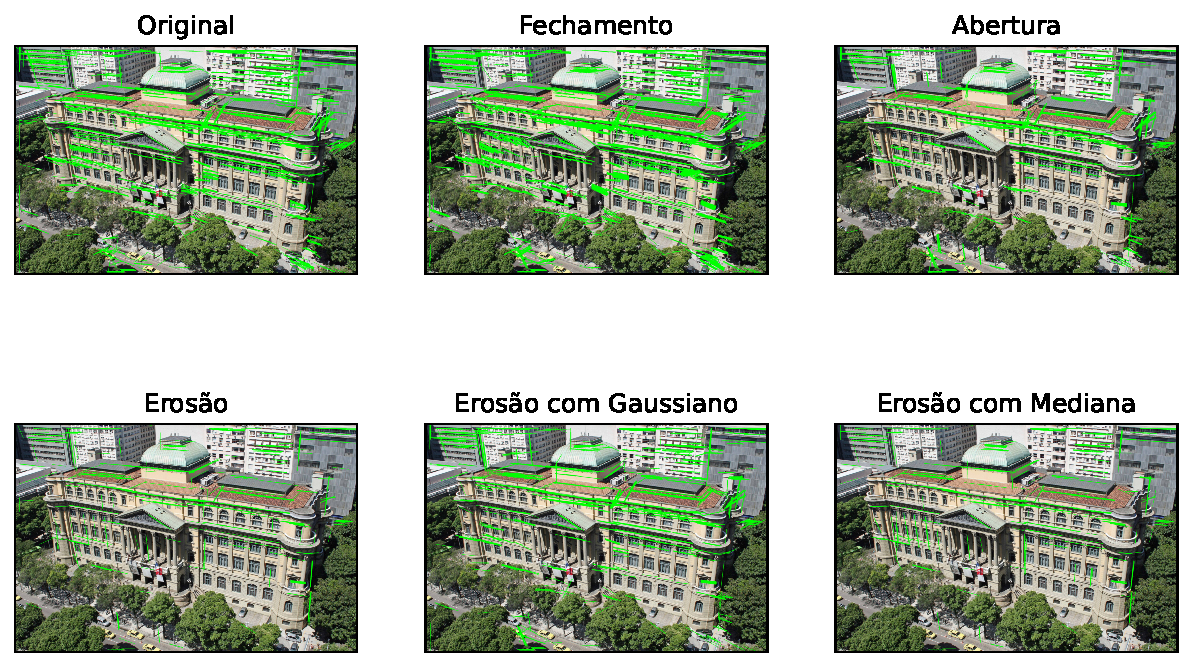
\includegraphics[scale=0.6]{houghP.pdf}
\caption{Imagem original e resultado da aplicação da transformada de Hough probabilística.}
\label{fig:hough}
\end{figure}

Nota-se que a transformada de Hough probabilística consegue detectar as arestas que compõem os edifícios, entretanto, ela não consegue detectar todas as arestas e algumas arestas são detectadas mais de uma vez. Por isso, foi testado um método mais robusto que será discutido na próxima subseção: a detecção de segmentos de retas.

\subsection{Detecção de segmentos a partir de pontos}

Para a detecção de segmentos, foi utilizada a implementação do Line Segment Detector \cite{opencv_manual} pela biblioteca opencv \cite{opencv_library} na interface Python. O LineSegmentDetector é um algoritmo de visão computacional que é capaz de detectar segmentos de retas em uma imagem, seu algoritmo é baseado em uma técnica de agrupamento de pontos chamada de \textbf{Progressive Probabilistic Hough Transform (PPHT)} \cite{matas2000robust}. O O algoritmo PPHT utilizado pelo Line Segment Detector opera de forma hierárquica, refinando gradualmente o processo de detecção de linha. Ele começa analisando a imagem em baixa resolução e aumenta progressivamente a resolução, permitindo a detecção de segmentos de linha grosseiros e finos. A desvantagem é que ele detecta todos os segmentos de linha selecionados pelo HED, incluindo os ruídos, e, por isso, é necessário desconsiderar os segmentos de linha que não são relevantes para a aplicação. A figura \ref{fig:lsd} mostra a imagem original e o resultado da aplicação do Line Segment Detector:

\begin{figure}
\centering
\includegraphics[scale=0.60]{lsd.pdf}
\caption{Imagem original e resultado da aplicação do Line Segment Detector.}
\label{fig:lsd}
\end{figure}


\section{Classificação de segmentos}

Nota-se que o algoritmo de detecção de segmentos de retas do opencv obteve bom resultado em relação a transformada de Hough probabilística, sendo assim, o cálculo dessa seção será baseado nos segmentos de retas deste algoritmo. Nesta seção será discutido como classificar os segmentos de retas matematicamente a partir dos pontos extremos de cada segmento. A próxima subseção discutirá as propriedades matemáticas dos pontos de fuga e como utilizar essas propriedades para classificar os segmentos de retas de forma computacionalmente eficiente.

\subsection{Modelo de câmera pinhole}

O modelo matemático mais simples para representar a fotografia de uma cena é o modelo de câmera pinhole. Esse modelo é baseado na projeção de perspectiva, onde os raios de luz que saem de um ponto da cena e atingem o plano da imagem são representados por retas que passam pelo centro de projeção da câmera. Esse modelo despreza as distorções óticas da lente da câmera e considera que a câmera está alinhada com o plano da imagem, ou seja, a câmera está perpendicular ao plano da imagem, esse mesmo modelo é utilizado pelo trabalho do Tomás Ferranti \cite{Ferranti2021}.

Considerando esse modelo, tem-se cada ponto da cena é representado no plano projetivo por um raio de luz que passa pelo centro de projeção da câmera e atinge o plano da imagem. O plano projetivo é um plano bidimensional, um subespaço afim de dimensão 2, que contém a imagem projetada pela luz que passou pelas lentes da câmera. A principal propriedade do plano projetivo que é interessante para essa aplicação são os pontos de fuga. Os pontos de fuga são os pontos de intersecção de retas paralelas no $R^3$ que são projetadas em retas concorrentes no plano projetivo. Como axioma, todas as retas paralelas no $R^3$ se intersectam em um ponto no plano projetivo, nem que este seja no infinito. Um ponto de fuga é dito degenerado quando ele está no infinito.
% \subsection{Axiomas do plano projetivo}

% \begin{axiom}

% Dados três pontos distintos $A$, $B$ e $C$ não colineares, existe uma única reta que passa por esses três pontos.

% \end{axiom}

% \begin{axiom}

%     Os pontos de fuga são os pontos de intersecção de retas paralelas no $R^3$ que são projetadas em retas concorrentes no plano projetivo.

% \end{axiom}

% \begin{axiom}

%     Dados dois pontos distintos $A$ e $B$, existe uma única reta que passa por esses dois pontos.

% \end{axiom}

% axioma de que todas as retas paralelas no $R^3$ se intersectam em um ponto no plano projetivo.


% A figura \ref{fig:pinhole} mostra o modelo de câmera pinhole.

% Uma fotografia tradicional é uma representação bidimensional da realidade. Fisicamente, o obturador controla a quantidade de luz que entre pelas lentes da câmera e, quando a luz atinge o sensor, ela é projetada no plano focal da câmera. O plano focal é um plano bidimensional que contém a imagem projetada pela luz que passou pelas lentes da câmera. Matematicamente, os objetos da cena tridimensional são projetadas no plano projetivo, que é um plano bidimensional, um subespaço afim de dimensão 2, que contém a imagem projetada pela luz que passou pelas lentes da câmera. A principal propriedade do plano projetivo que é interessante para essa aplicação são os pontos de fuga. Os pontos de fuga são os pontos de intersecção de retas paralelas no $R^3$ que são projetadas em retas concorrentes no plano projetivo. Como axioma, todas as que são retas paralelas no $R^3$ se intersectam em um ponto no plano projetivo. 

\subsection{Classificação de acordo com os pontos de fuga}


Os dados dessa aplicação são fotografias de edifícios, e, esses dados possuem algumas hipóteses que serão utilizadas para classificar os segmentos de retas. A primeira hipótese é que os edifícios possuem faces aproximadamente retas, ou seja, os segmentos de retas que compõem as arestas dos edifícios são aproximadamente retos. A segunda hipótese é que os edifícios possuem faces que são perpendiculares entre si, ou seja, os segmentos de retas que compõem as arestas dos edifícios são perpendiculares entre si. A terceira hipótese é que a câmera está externa ao edifício. A quarta hipótese é que um dos pontos de fuga é aproximadamente degenerado verticalmente, ou seja, a câmera está aproximadamente alinhada com a base do edifício. Todas as hipóteses são razoáveis considerando os dados alvo: fotografias históricas de faxadas de edifícios.

Considerando a representação digitais binárias, como ocorre com a imagem de saída da etapa da etapa de detecção de arestas, a origem $(0,0)$ do plano cartesiano está no ponto superior esquerdo com o eixo $x$ crescendo para a direita e o eixo $y$ crescendo para baixo. Então, a equação da inclinação da reta que passa pelos pontos $(x_1,y_1)$ e $(x_2,y_2)$ é dada por:

$$ 
m = \frac{y_2-y_1}{x_2-x_1}
$$

Podemos obter o ângulo $\theta$ que a reta faz com o eixo $x$ por meio da função arco tangente:

$$
\theta = \arctan(m)
$$

A hipótese de que a câmera está alinhada com a base do edifício, ou seja, um dos pontos de fuga é aproximadamente degenerado verticalmente, implica que a reta que passa pelo ponto $(x_1,y_1)$ e $(x_2,y_2)$ é aproximadamente vertical, ou seja, o coeficiente angular $m$, em módulo, tende ao infinito. Sendo assim, foi definido um parâmetro $alpha$ tal que se $m > alpha$ então a reta é aproximadamente vertical e esta foi classificado com o ponto de fuga vertical de classe 0. Por padrão o parâmetro $alpha$ foi definido como $alpha=2$, arbitrariamente. Os demais seguimentos foram classificados em mais dois grupos de acordo com os pontos de fuga restantes, para essa divisão, houve a subdivisão do problema em 3 casos:

\begin{enumerate}
    \item Existe um ponto de fuga horizontal degenerado, ou seja, a câmera está aproximadamente alinhada com a lateral do edifício.
    \item Não existe um ponto de fuga horizontal degenerado, mas, os pontos de fugas estão distantes entre si e distantes do centro da imagem.
    \item Não existe um ponto de fuga horizontal degenerado, mas, os pontos de fugas estão próximos entre si e próximos do centro da imagem.
\end{enumerate}

\subsubsection{Ponto de fuga horizontal degenerado}

A figura \ref{fig:salvador} de \cite{salvador} é um example de fotografia com o ponto de fuga horizontal degenerado. Nesse caso, a câmera está aproximadamente alinhada com a lateral do edifício, ou seja, a reta que passa pelo ponto $(x_1,y_1)$ e $(x_2,y_2)$ é aproximadamente horizontal, ou seja, o ângulo, em módulo, tende a zero. Sendo assim, foi definido um parâmetro $beta$ tal que se $\theta < beta$ então a reta é aproximadamente horizontal e esta foi classificado com o ponto de fuga horizontal degenerado de classe 1. Por padrão o parâmetro $beta$ foi definido como $beta=0.1$, arbitrariamente. Os demais seguimentos foram classificados na classe 2, que é a classe restante.

\begin{figure}[H]
\centering
\includegraphics[scale=0.20]{salvador.jpg}
\caption{Exemplo de imagem com ponto de fuga horizontal degenerado.}
\label{fig:salvador}
\end{figure}

Após aplicar o algoritmo nesse caso foi obtido o seguinte resultado na figura \ref{fig:horizontal}:

\begin{figure}[H]
    \centering
    \includegraphics[scale=0.80]{horizonte2.pdf}
    \caption{Resultado final da classificação de segmentos de retas no caso de ponto de fuga horizontal degenerado.}
    \label{fig:horizontal}
    \end{figure}
end{figure}

\subsubsection{Pontos de fuga distantes}

Caso os pontos de fuga estejam distantes da imagem, então, as retas originalmente paralelas, possuem uma inclinação ligeiramente diferente, pois elas irão se encontrar em um dos pontos de fuga distantes. Neste caso, como a câmera está externa ao edifício e os ângulos entre as faces do edifício são aproximadamente retos então, os ângulos dessas retas no plano projetivo são ângulos agudos por conta dos pontos de fugas estarem distantes. Sendo assim, o ângulo em relação ao eixo $x$ da reta que passa pelos pontos $(x_1,y_1)$ e $(x_2,y_2)$ foi classificado para a classe um se $\theta < 0$ e para a classe 2 se $\theta > 0$, pois, necessariamente, um dos pontos de fuga é ascendente e o outro é descendente dado que os ângulos são agudos. A figura \ref*{fig:normal} mostra um exemplo de pontos de fuga distantes classificados de acordo com essa lógica.

\begin{figure}[H]
    \centering
    \includegraphics[scale=0.80]{normal.pdf}
    \caption{Exemplo de imagem com ponto de fuga distantes}
    \label{fig:normal}
\end{figure}


\subsubsection{Pontos de fuga próximos}

Por outro lado, caso os pontos de fuga estejam próximos da imagem, então, as retas originalmente paralelas, possuem uma inclinação muito diferente, pois elas irão se encontrar em um dos pontos de fuga próximos. Neste caso, como a câmera está externa ao edifício e os ângulos entre as faces do edifício são aproximadamente retos então, os ângulos dessas retas no plano projetivo são ângulos obtusos já que os pontos de fuga estão próximos. Sendo assim, os pontos de fuga se encontram com seu $y$ entre essas retas, portanto, a partir da altura $h$ do ponto de fuga, foi-se necessário inverter a classificação das retas, ou seja, o ângulo em relação ao eixo $x$ é classificado para a classe 1 se $\theta < 0$ e se $y_i < h^*$ ou se $\theta > 0$ e se $y_i > h^*$ e para a classe 2 caso contrário A figura \ref{fig:proximos} mostra um exemplo de pontos de fuga próximos classificados de acordo com essa lógica.

\begin{figure}[H]
    \centering
    \includegraphics[scale=0.60]{inverse.pdf}
    \caption{Exemplo de imagem com ponto de fuga próximos}
    \label{fig:proximos}
\end{figure}

\subsection{Algoritmo de classificação}

Após os comentários em relação a lógica da classificação, o algoritmo de classificação é apresentado a seguir:

\begin{algorithm}
    \small \small \small \small
    \caption{Funções auxiliares}
    \begin{algorithmic}[1]
    
    \Function{calcula\_inclinacao}{pontos}
        \State $x1, y1, x2, y2 \gets$ pontos 
        \State $m \gets \dfrac{y2 - y1}{x2 - x1}$
        \State \Return $m$ 
    \EndFunction
    
    \Function{calcula\_angulo}{pontos=None, m=None}
        \If{$\text{type}(m) == \text{None}$}
            \State $m \gets \text{calcula\_inclinacao}(pontos)$
        \EndIf
        \State $\text{angulo} \gets \text{np.arctan}(m)$
        \State \Return angulo
    \EndFunction
    
    \Function{vetor\_inclinacao}{pontos}
        \State func $\gets \lambda x: \text{calcula\_inclinacao}(x)$
        \State \Return $\text{np.apply\_along\_axis}(\text{func}, 1, \text{pontos})$
    \EndFunction
    
    \Function{vetor\_angulo}{pontos}
        \State func $\gets \text{np.vectorize}(\text{calcula\_angulo})$
        \State $m \gets \text{func}(pontos)$
        \State \Return $m$
    \EndFunction
    
    \Function{vetor\_angulo\_dado\_m}{m}
        \State $\text{angulo} \gets \text{calcula\_angulo}(m=m)$
        \State \Return angulo
    \EndFunction
\end{algorithmic}
\end{algorithm}

\begin{algorithm}
\begin{algorithmic}[2]
    \small \small \small \small
    \caption{Função principal de classificação de segmentos de retas}
    \Function{cluster\_final}{n\_cluster=3, alpha=2, image\_path='t', image\_opencv=None, swap=False, swapPercent=0.75}
    \If{$\text{image\_opencv} \neq \text{None}$}
        \State lines $\gets \text{getLines}(\text{image\_opencv=image\_opencv})$
    \Else
        \State lines $\gets \text{getLines}(\text{image\_path})$
    \EndIf
    \State lines $\gets$ lines$[:,0:4]$
    \State $m \gets \text{vetor\_inclinacao}(\text{lines})$
    \State angulo $\gets \text{vetor\_angulo\_dado\_m}(m)$
    \State class0, class1 $\gets \text{filtro\_inclinacao}(m, \alpha)$
    \State class0 $\gets \text{np.array}(class0)$
    \State class1 $\gets \text{np.array}(class1)$
    \State labels $\gets \text{cluster\_lines\_angulo}(\text{angulo[class1]}, \text{lines[class1]}, n\_cluster, \text{swap=swap}, \text{swapPercent=swapPercent})$
    \State allClass $\gets \text{np.zeros}([\text{lines.shape}[0]])$
    \State allClass[class0] $\gets 0$
    \State allClass[class1] $\gets \text{labels} + 1$
    \State \Return allClass, lines
\EndFunction

\end{algorithmic}
\end{algorithm}

\begin{algorithm}
    \small \small \small \small
\begin{algorithmic}[3]
    \caption{Função de clusterização de segmentos de retas de acordo com o ângulo para as retas não verticais}

\Function{cluster\_lines\_angulo}{angulo, lines, n\_clusters=2, beta=0.1, swap=False, swapPercent=0.75}
    \State count $\gets 0$
    \For{$i \gets 0$ to $\text{angulo.shape}[0]$}
        \If{$\left|\text{angulo}[i]\right| \leq \text{beta}$}
            \State count $\gets$ count $+ 1$
        \EndIf
    \EndFor
    \State \Call{print}{$\dfrac{\text{count}}{\text{angulo.shape}[0]}$}
    \If{$\dfrac{\text{count}}{\text{angulo.shape}[0]} > 0.25$}
        \State values $\gets$ []
        \For{$i \gets 0$ to $\text{angulo.shape}[0]$}
            \If{$\left|\text{angulo}[i]\right| \leq \text{beta}$}
                \State values.\text{append}(0)
            \Else
                \State values.\text{append}(1)
            \EndIf
        \EndFor
        \State \Return \text{np.array}(values)
    \EndIf

    \State $h \gets \text{max}(\text{max}(\text{lines}[:,1]), \text{max}(\text{lines}[:,3]))$

    \State values $\gets$ []
    \For{$i \gets 0$ to $\text{angulo.shape}[0]$}
        \If{$\text{angulo}[i] > 0$}
            \If{not \text{swap}}
                \State values.\text{append}(0)
            \ElsIf{$\text{lines}[i,1] > h \times \text{swapPercent}$ or $\text{lines}[i,3] > h \times \text{swapPercent}$}
                \State values.\text{append}(1)
            \Else
                \State values.\text{append}(0)
            \EndIf
        \Else
            \If{not \text{swap}}
                \State values.\text{append}(1)
            \ElsIf{$\text{lines}[i,1] > h \times \text{swapPercent}$ or $\text{lines}[i,3] > h \times \text{swapPercent}$}
                \State values.\text{append}(0)
            \Else
                \State values.\text{append}(1)
            \EndIf
        \EndIf
    \EndFor
    \State \Return \text{np.array}(values)
\EndFunction
\end{algorithmic}
\end{algorithm}
% Notamos que ainda sobra

% \centering
% %left bottom right top
% %\includegraphics[trim=10mm 00mm 00mm 00mm, scale=0.40]{tabela.pdf}
% \begin{center}
% Figura 1: tabela.
% \end{center}

% \begin{figure}[H]
% \centering
% %left bottom right top
% %\includegraphics[trim=10mm 00mm 00mm 00mm, scale=0.40]{tabela.pdf}
% \begin{center}
% Figura 2: tabela.
% \end{center}
% \end{figure}

% \newpage
% \subsubsection{yy}

% yy

% % \[\left\{ 
% \begin{align*}
% f_{i}(x) = (10x + 100), \qquad \text{(1)} \tag{1}\\
% f_{ii}(x) = (20x + 200), \qquad \text{(2)} \tag{2} \\
% f_{iii}(x) = (30x + 300), \qquad \text{(3)} \tag{3} \\
% \end{align*} %\right.\]

% xx

% \begin{align*}
% Vm_{i}(p,l) = ((-1.9141)p + 49.466)l + ((199.51)p - 10795.0), \text {$l$=0} \tag{4}
% \end{align*}

% \begin{align*}
% f_{n}(y) = \frac{y}{1000}, \tag{5}
% \end{align*}

% \subsection{xx}

% xx

% %\[\left\{
% \begin{align*} 
% Funcao_{i}(p) = \gamma + \delta p + \theta p^2 + \omega p^3, \qquad \qquad \qquad \qquad \qquad \qquad \qquad \qquad \text{(6)} \tag{6} \\
% \end{align*} %\right.\]

% \newpage
% \section{Resultados Esperados}

% Nesta seção serão apresentados os resultados esperados...

% \subsection{xx}

% xx

\newpage
\section{Referências}

% [1] a.

% \noindent [2] b.

% \noindent [3] c.

% \noindent [4] d.

\printbibliography

\end{document}